%%%%%%%%%%%%%%%%%%%%%%%%%%%%%%%%%%%%%%%%%%%%%%%%%%%%%%%%%%%%%%%%%%%%
%% I, the copyright holder of this work, release this work into the
%% public domain. This applies worldwide. In some countries this may
%% not be legally possible; if so: I grant anyone the right to use
%% this work for any purpose, without any conditions, unless such
%% conditions are required by law.
%%%%%%%%%%%%%%%%%%%%%%%%%%%%%%%%%%%%%%%%%%%%%%%%%%%%%%%%%%%%%%%%%%%%

\documentclass{beamer}
\usetheme[logo=figures/McMasterLogo,faculty=phil]{fibeamer}
\usepackage[utf8]{inputenc}
\usepackage[
  main=english, %% By using `czech` or `slovak` as the main locale
                %% instead of `english`, you can typeset the
                %% presentation in either Czech or Slovak,
                %% respectively.
  czech, slovak %% The additional keys allow foreign texts to be
]{babel}        %% typeset as follows:
%%
%%   \begin{otherlanguage}{czech}   ... \end{otherlanguage}
%%   \begin{otherlanguage}{slovak}  ... \end{otherlanguage}
%%
%% These macros specify information about the presentation
\title{\normalsize PhD SUPERVISORY COMMITTEE MEETING REPORT \\
        Aug. $30^{th}$ 2017} %% that will be typeset on the
\subtitle{Ph.D Candidate: Curtis D'Alves} %% title page.
\author{Supervisors: Dr. Christopher Anand, Dr. Wolfram Kahl}
%% These additional packages are used within the document:
\usepackage{ragged2e}  % `\justifying` text
\usepackage{booktabs}  % Tables
\usepackage{tabularx}
\usepackage{tikz}      % Diagrams
\usetikzlibrary{calc, shapes, backgrounds}
\usepackage{amsmath, amssymb}
\usepackage{url}       % `\url`s
\usepackage{listings}  % Code listings
\usepackage{float}
\usepackage{caption}


\frenchspacing

\begin{document}
  \frame{\maketitle}

  %\AtBeginSection[]{% Print an outline at the beginning of sections
  %  \begin{frame}<beamer>
  %    \frametitle{Table of Contents}
  %    \tableofcontents[currentsection]
  %  \end{frame}}

  \begin{darkframes}
%%%%%%%%%%%%%%%%%%%%%%%%%%%%%%%%%%%%%%%%%%%%%%%%%%%%%%%%%%%%%%%%%%%%%%%%%%%%%%%%%%%%%%%%%%%%%%%%%%%%%%%%%%%%%%%%
%%%%%%%%%%%%%%%%%%%%%%%%%%%%%%%%%%%%%%%%%%%%%%%%%%%%%%%%%%%%%%%%%%%%%%%%%%%%%%%%%%%%%%%%%%%%%%%%%%%%%%%%%%%%%%%%
%%%%%%%%%%%%%%%%%%%%%%%%%%%%%%%%%%%%%%%%%%%%%%%%%%%%%%%%%%%%%%%%%%%%%%%%%%%%%%%%%%%%%%%%%%%%%%%%%%%%%%%%%%%%%%%%
\section{Specific Accomplishments To Date}
\begin{frame}{Specific Accomplishments To Date}
\begin{itemize}
 \item Completed CAS 705 - Computability and Complexity \\
 (1/4 700 courses) { \bf \color{green} (Winter 2017)} \\
 \qquad \\
 \item Completed Comprehensive Examination { \bf \color{green} (May 26, 2017)} \\
 \qquad \\
 \item Presented Research on Instruction Scheduling Algorithms at IBM's TechConnect Poster Exhibition { \bf \color{green} (May 2nd 2017)} \\
 \qquad \\
\end{itemize}
\end{frame}

\begin{frame}{Specific Accomplishments To Date}
\begin{itemize}
 \item Co-authored paper "Using Elm to Introduce Algebraic Thinking to K-8 Students" on research into education using functional programming and presented it at TFPIE conference at the University of Kent { \bf \color{green} (June 29th 2017)} \\
 \qquad \\
 \item Co-authored paper "Accelerating Poly1305 Cryptographic Message Authentication on the Z14" accepted into IBM's CASCON 2017, which detailed my contributions to the work via performance optimised instruction scheduling of code used { \bf \color{green} (August 2017)}
\end{itemize}
\end{frame}


\section{My Research}
\begin{frame}{My Research}
    \qquad \\
    \qquad \\
    \begin{itemize}
        \item IBM CAS Project - Research into Instruction Scheduling Algorithms for Vector (SIMD) Libraries, on Out-of-order execution architectures \\
        \qquad \\
        \qquad \\
        \qquad \\
        \pause
        \item Commonly used heuristics in conventional compilers are efficient but generate far from optimal schedules  \\
    \end{itemize}
\end{frame}

\begin{frame}{My Research}
    \qquad \\
    \qquad \\
    \begin{itemize}
        \item Currently, little research has been made into consideration of register allocation during scheduling (known NP-Hard problem) \\
        \qquad \\
        \qquad \\
        \pause
        \item In attempt to obtain near-optimal schedules in reasonable amounts of time, we're developing a continuous optimization model that can encompass many overlapping heuristics for scheduling and register allocation
    \end{itemize}
\end{frame}

\begin{frame}{Relaxed Continuous Optimization based Scheduling}
    Per Instruction $i$, perform a relaxation of scheduled position to dispatch and completion times $t_i$, $b_i$
    \begin{align*}
    \text{\color{cyan} Objective Variables \qquad} & t_i, b_i, f_i:& \mathbb{R} \\
    \text{\color{cyan} Constants \qquad} & \textrm{II} :& \mathbb{R} \\
    \text{\color{cyan} Indicator Function \qquad} & \mathsf{IN} :& \mathbb{R} \rightarrow \mathbb{R} \\
    & t_i :& \text{dispatch time} \\
    & b_i :& \text{completion time} \\
    & f_i :& \text{FIFO use } 0 \leq f_i \leq 1 \\
    & \textrm{II} :& \text{iteration interval} \frac{\# instructions}{dispatches/cycle} \\
    \end{align*}
   
\end{frame}

\begin{frame}{Relaxed Continuous Optimization based Scheduling}
    \begin{align}
    \text{\color{cyan} Hard Constraints \qquad}  & t_i + \epsilon \leq t_j  & \hspace{-9em} \forall i,j \; . \; i \rightarrow j \\
								 & 0 \leq t_i \leq b_i \leq \#\text{stages} \cdot \textrm{II}  & \\
								 & b_i + \epsilon \leq t_i + \textrm{II} \\
    \text{\color{cyan} Objective Function \qquad}   & \text{min} \sum_{i} (b_i - t_i) + \text{Penalties}
    \end{align}
    
    {\bf \color{green} Key Idea:} Encode choice heuristics as penalties, adjust preference between heuristics by scaling
\end{frame}

\begin{frame}{Relaxed Continuous Optimization based Scheduling}

    {\bf \color{green} Example:} Floating Point Dispatch Penalty, using Indicator Function  \\
    \qquad $ \sum_{(t_i, t_j) \in FP \times FP} \mathsf{IN}(|t_i - t_j|)$ 
    \begin{figure}
        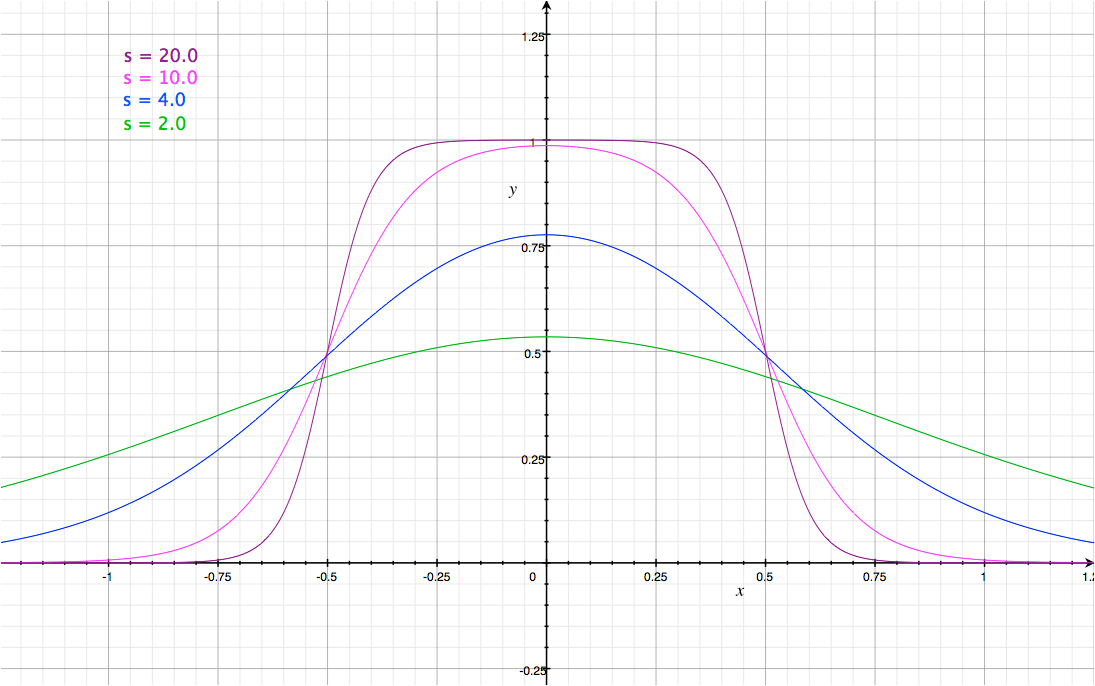
\includegraphics[scale=0.2]{figures/sigmoid}
        \caption{\textrm{IN} - Altered Sigmoid Indicator Function}
    \end{figure}

\end{frame}

\begin{frame}{General Progress in Current Research}

\begin{itemize}
 \item Developed a non-linear programming model for instruction scheduling 
 \pause
 \item Implemented code generation software, specifically for generating AMPL code corresponding to above model 
 \pause
 \item Tested implementation on IBM MASS library functions, achieved a working implementation of Vector cosine with a estimated 20\% speedup over previous implementations
 \pause
 \item Modified code generator to assist with optimising inlined Z assembly code in GoLang modules
 \pause
 \item Tested implementation of inlined Z assembly code in the Z14 GoLang compiler on a Poly1305 encryption algorithm with a moderate speedup of 7\%
\end{itemize}

\end{frame}

  \end{darkframes}

\end{document}
